% \begin{figure}[ht]
%     \centering
%     \subfloat[QR Code]{{
\includegraphics[width=0.185\textwidth]{images/qr_code_example_cropped.png} }} %https://www.qr-code-generator.com/wp-content/themes/qr/new_structure/markets/core_market_full/generator/dist/generator/assets/images/websiteQRCode_noFrame.png
%     % \hspace{0.001cm}
%     \subfloat[ARTag]{{
\includegraphics[width=0.185\textwidth]{images/artag_example_cropped.png}}}%https://www.researchgate.net/profile/Martin_Rehak2/publication/314259443/figure/fig44/AS:668970931724296@1536506507808/An-example-of-ARTag-fiducial-marker.jpg
%     \hspace{0.001cm}
%     \subfloat[April Tag]{{
\includegraphics[width=0.185\textwidth]{images/apriltag_example_cropped.png}}} %https://cdn.shopify.com/s/files/1/0803/9211/files/tag36h10_0_large.png?v=1487041161
%     \hspace{0.05cm}
%     \subfloat[WhyCon]{{
\includegraphics[width=0.185\textwidth]{images/whycon_example.png}}} %
%     \hspace{0.05cm}
%     \subfloat[WhyCode]{{
\includegraphics[width=0.185\textwidth]{images/whycode_example.png}}} %https://encrypted-tbn0.gstatic.com/images?q=tbn:ANd9GcQzLY0TeIWzl7sMrlLTahfMMMiKp6CjL6GcjzhxMYpN10s8MbGK&s
%     \caption{Common fiducial markers.}
%     \label{fig:fiducial_markers}
% \end{figure}

\begin{figure}[ht]
    \centering
    \begin{subfigure}[b]{0.16\textwidth}
        \centering
        
\includegraphics[width=\textwidth]{images/qr_code_example_cropped.png}
        \caption{QR Code}
        \label{subfig:qr_code}
    \end{subfigure}
    \begin{subfigure}[b]{0.16\textwidth}
        \centering
        
\includegraphics[width=\textwidth]{images/artag_example_cropped.png}
        \caption{AR Tag}
        \label{subfig:ar_tag}
    \end{subfigure}
    \begin{subfigure}[b]{0.16\textwidth}
        \centering
        
\includegraphics[width=\textwidth]{images/apriltag_example_cropped.png}
        \caption{April Tag}
        \label{subfig:apriltag}
    \end{subfigure}
    \begin{subfigure}[b]{0.16\textwidth}
        \centering
        
\includegraphics[width=\textwidth]{images/aruco.png}
        \caption{ArUco}
        \label{subfig:aruco}
    \end{subfigure}
    \begin{subfigure}[b]{0.16\textwidth}
        \centering
        
\includegraphics[width=\textwidth]{images/whycon_example.png}
        \caption{WhyCon}
        \label{subfig:whycon}
    \end{subfigure}
    \begin{subfigure}[b]{0.16\textwidth}
        \centering
        
\includegraphics[width=\textwidth]{images/whycode_example.png}
        \caption{WhyCode}
        \label{subfig:whycode}
    \end{subfigure}
    \caption{Common fiducial markers.}
    \label{fig:fiducial_markers}
\end{figure}

Fiducial markers, examples of which are shown in Figure \ref{fig:fiducial_markers}, have been used in computer vision in the recent past for computationally cheap, unambiguous determination of an object's orientation and position in space. These markers are easy to produce, as they are planar and can typically be printed in a range of sizes on a normal sheet of paper and be fastened to whichever surface needs to be identified. This makes fiducial markers a convenient solution for enabling a drone to precisely identify and approach a landing pad that is labeled with a fiducial marker. A well known fiducial marker is the QR Code, which is able to store much more data than typical fiducial markers in the robotics domain. However, this high data density gives the QR Codes an intricate design which is prohibitively difficult to fully process in many robotics applications wherein pose distortion, motion blur, and varying light conditions may obscure the image.

Within the robotics domain, fiducial markers tend to carry less data than QR Codes while being more robustly identifiable in a variety of conditions. Many different fiducial markers and corresponding identification systems are available, such as ARTag, AprilTag, WhyCon, and WhyCode. ARTag, a shortened form of \textit{Augmented Reality} Tag, is a bi-tonal, square symbol consisting of a solid background with a 6x6 grid of high contrast interior cells which can encode 2002 different identifying codes \cite{Fiala:2005:AFM:1068508.1069138}. One significant issue in applying ARTag is that its detection algorithm is not public, which makes further development difficult or impossible. Only general information about the detection algorithm for ARTag is available.

AprilTag is a very similar fiducial marker to ARTag, with the principal difference being that it is open source. AprilTags use the same general form as ARTag: a black square with a 6x6 interior region of black or white squares which encode a binary sequence and ultimately denote an identifier. The detection algorithm analyzes a given image using the image's gradient and attempts to find four-sided dark regions. The detection algorithm has, by design, a low false-negative rate and a high false-positive rate, and it is therefore coupled with a decoding algorithm that verifies whether the detected squares form a proper AprilTag identifier. While this coupling does increase the accuracy of reported AprilTag detections, it also means that an accurate reading of the identifier is a necessary part of the detection, which makes the AprilTag harder to detect in noisy conditions or from long distances \cite{apriltag_paper}. Still, AprilTags have been used with high success in a wide variety of robotics applications to allow vision systems to identify and orient objects in 3 dimensional space. AprilTag detectors have been made open source and are freely available in both Python and C++.

Aruco is another fiducial marker following the black and white square paradigm of AR Tag and April Tag \cite{aruco_orig}. It has a black border and a configurable number of ID bits which determines the black and white interior pattern. Its algorithm works by first detecting and extracting the most prominent contours in its input image. Then, it analyzes the inner region of the contours in order to extract the marker's ID code. The image is converted to black and white, and each interior square region receives a value of 0 or 1 corresponding to the color of the majority of its pixels. The black border is a necessary part of the marker, so a check for this feature functions as a first rejection test. Then, the detected marker ID is compared to a dictionary of set IDs. If a corresponding ID does not exist in the dictionary, error correction is applied to determine whether the detected ID is within some distance to an existing ID. If a corresponding ID can then be found, the marker is detected and its pose is estimated.

WhyCon is a circular marker developed by Nitsche et~al.\@ at the University of Buenos Aires in 2015 \cite{whycon_paper}. The simple marker consists of an outer black circle whose center is covered by an inner white circle. The simplicity of the design makes the marker easy to identify even with high perspective distortion - such as, for example, when viewing it from an extreme angle. The detection algorithm is simple and computationally cheap. The relevant image is first searched for dark pixels, and flood-fill is then used to detect a contiguous region of dark pixels. The centroid of the dark region is then the starting point for a second search of a light region, which is flood-filled in a similar way. If the inner region is indeed lighter than the darker region, then the elliptical properties of the symbol are verified. Specifically, the detection algorithm verifies that the semi-axes and centroids of each region are roughly aligned, and that the ratio of the pixel areas of each region is roughly as expected in the known WhyCon tag. When applied to a video feed, the search for the black and white regions in frame $n$ begins at the pixel positions where those regions were found in frame $n-1$, which decreases the computational load of the algorithm. A WhyCon marker's position and orientation in 2 dimensions can be detected very quickly. However, the drawback to WhyCon is that not all components of its rotational orientation cannot be determined, since it has full radial symmetry. Further, multiple WhyCon markers cannot be distinguished from one another because they do not contain identifiers. Still, it remains a useful and cheap marker. The WhyCon infrastructure is provided in a ROS module and is available in the open source community.


\begin{figure}
    \centering
    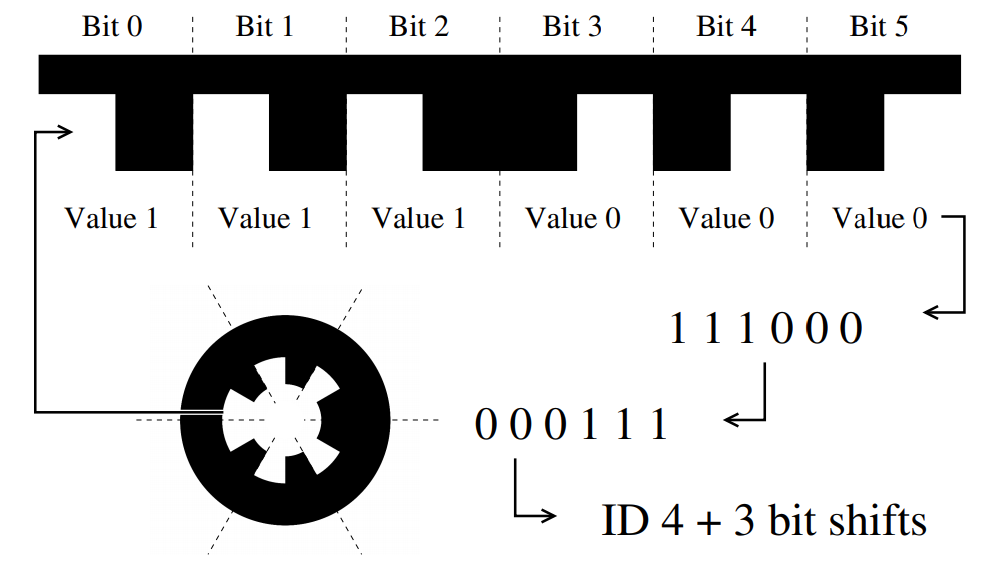
\includegraphics[width=0.5\textwidth]{images/whycode_manchester_explanation.png}
    \caption{The WhyCode marker and ``Necklace'' encoding, from Lightbody et~al.\@.}
    \label{fig:whycode_manchester_explanation}
\end{figure}


As an extension to WhyCon, Lightbody et~al.\@ developed the WhyCode marker in 2017. WhyCode uses the characteristic exterior, circular, black region and interior, circular, white region, but also uses a ``Necklace'' encoding, which is a Manchester encoding of a binary value that is wrapped around the interior white region. This is illustrated in Figure \ref{fig:whycode_manchester_explanation} (from \cite{whycode_paper}). This property of WhyCode markers allows them to break the radial symmetry of WhyCon markers, and also allows them to be distinguished from each other. Some patterns do still have radial symmetry with one another, as some WhyCode IDs have the same shape rotated by some angle. WhyCode markers use essentially the same flood-fill and ellipse-based detection system that WhyCon markers use, but with the added component of a Necklace decoder. The radial asymmetry allows the full spacial pose of the marker to be determined - including the rotational orientation (with some ambiguity based on ID, although this is conceptually able to be overcome). This added benefit makes the marker more appealing than its WhyCon predecessor, while still retaining almost all of the WhyCon computational cheapness. Furthermore, the detection of WhyCode markers is independent from the decoding of the Necklace. This is important because it allows the marker to still be detected in cases where its more intricate encoding is obscured, such as in scenarios of high motion blur or extreme perspective distortion. It also gives the WhyCode marker an edge over the widely-used AprilTag, which must be detected simultaneously with its encoding.


